\documentclass{cumcmthesis}
% \documentclass[withoutpreface,bwprint]{cumcmthesis} %去掉封面与编号页,电子版提交的时候使用。


\usepackage[framemethod=TikZ]{mdframed}
\usepackage{algorithm}
\usepackage{algorithmic}
\usepackage{placeins}
\usepackage{multirow}
\usepackage{url}   % 网页链接
\usepackage{subcaption} % 子标题
\title{多波束测线问题模型的建立和优化}
\tihao{B}
\baominghao{202319058027}
\schoolname{香港中文大学(深圳)}
\membera{陈希}
\memberb{薛中凯}
\memberc{张树晗}
\supervisor{吴均峰}
\yearinput{2023}
\monthinput{9}
\dayinput{10}

\begin{document}
 \maketitle


 \begin{abstract}
针对多波束测线问题,本文从相关理论入手,分析了问题的几何特征,给出了一定误差下具有实践价值的优化模型,并根据探测情形的复杂度,给出了针对性的具体优化解决方案,具有良好的普适性,且有较高的效率。

对于\textbf{问题1},我们给出了两种解法。一种解法是充分利用三角形的几何特性,通过\textbf{正弦定理}列出三角方程进行求解,然后再进一步研究动态情况下变量之间的关系;另一种充分利用波束变动前后的变化量和不变量,抓住共顶点的一组\textbf{相似三角形},最终列出等比关系进行求解。在这个过程中,我们还根据具体情况给出了坡面情况下\textbf{重叠率}的定义和定量表示,为后续更加一般情况的分析打下基础。

对于\textbf{问题2},我们充分吸取了\textbf{转化与化归}的思想,分析更复杂模型变化的实质在于坡面角度的变量,因此提出了\textbf{等效坡面角}的概念,接着可以直接转化为问题一,较为清晰、简洁地给出了相关模型特征。

对于\textbf{问题3},综合考虑方案的可行性和高效性,我们粗略讨论了两种可能的\textbf{测线走向}。在确定大致走向后,我们以之前提出的模型为基础,用\textbf{动态规划}的思想,在\textbf{迭代}的具体操作方法下由起始边界情况开始,在触发终止边界情况时结束。我们分别考虑了两种具体的\textbf{测量顺序},经过评估后结果基本一致,更加印证了方案的可靠性。根据题目所给数据,可以算到,从东向西一共有 34 条测线,总路程为 125936 米(68 海里);从西向东一共有 34 条测线,总路程为 125936 米(68 海里)。

对于\textbf{问题4},我们采取了\textbf{微元}的思想,将复杂的问题分成若干个子问题,并综合运用\textbf{可视化}的技巧和\textbf{Laplace算子}、\textbf{导数容忍度}等数理工具,将具体而复杂的平面划分为可算的几个区域,最终化归为问题3中的情形逐一解决。
我们根据数据特征,将复杂海底面划分为4个区域:
第一块区域一共有 43 条测线,总路程为107.5海里,遗漏率为11.50$\%$;第二块区域一共有 16 条测线,总路程为40.0 海里,遗漏率为 13.04$\%$;第三块区域一共有 28 条测线,总路程为56 海里,遗漏率为 10.79$\%$;第四块区域一共有 17 条测线,总路程为42.5 海里,遗漏率为 2.91$\%$。
\\
\\
\keywords{动态规划 \quad 转化与化归 \quad 等效法 \quad Laplace算子 \quad 线性回归 \quad 平面几何}
\end{abstract}


\tableofcontents

\newpage

\section{问题的背景和重述}
\subsection{问题的背景}
随着全球经济的快速发展和人类活动对海洋环境的日益增加,海洋的健康和可持续性成为了全球关注的焦点。在这样的背景下,对海底的准确测绘和了解变得尤为重要。这不仅可以保护珍贵的海洋生态系统,还确保我们的经济活动如海上交通、油气开采和海底建筑物的建设都能在安全和环境友好的基础上进行。

多波束测线(Multi-beam Echo Sounder,简称 MBES)作为一种先进的声纳测深系统,用于海底深度和形态的全覆盖测量。\cite{ref1}与传统的单波束声纳相比,多波束测线可以同时发送和接收多条声波束,从而在同一时间内覆盖更大的海底面积,达成高效率、高分辨率、广测量范围的优点。熟练进行测线布设与修改,对于多波束测线的应用具有重大实践意义。\cite{ref2}
\subsection{问题重述}
\textbf{总述:}在该问题中,多波束测深条带的覆盖宽度$W$受换能器开角 $\theta$ 和水深$D$影响而变化。当测线平行且海底平坦时,相邻条带的重叠率 $\eta = 1 - \frac dW$,其中 $d$ 是相邻两条测线的间距,$W$是条带的覆盖宽度。为确保测量便捷和数据完整性,相邻条带的重叠率应保持在$10\% \sim 20\%$。

然而,实际海底地形变化大。采用平均水深设计测线间隔时,虽然平均重叠率可满足要求,但在浅水区会漏测,影响质量。采用最浅水深设计测线间隔时,最浅处的重叠率符合要求,但深水区会有过多重叠,导致冗余数据增多,影响测量效率。因此,在下面分析问题时,需要综合考虑海底地形变化,选择适当的测线间隔以平衡测量质量和效率。

\textbf{问题1:}已知与测线方向垂直的平面和海底坡面的交线构成一条与水平面夹角,称为坡度 $\alpha$,需要建立多波束测深的覆盖宽度及相邻条带之间重叠率的数学模型。
同时,当特殊情况(多波束换能器的开角为 $120^\circ$,坡度为 $1.5^\circ$,海域中心点处的海水深度为 70 m)时,需要分别计算海水深度、覆盖宽度和与前一条测线的重叠率。

\textbf{问题2:}在考虑一个矩形待测海域时,假设测线的方向与水平面上海底坡面的法向的投影夹角为 $\beta$,需要构建一个数学模型来描述多波束测深覆盖宽度。
同时,当特殊情况(多波束换能器的开角为 $120^\circ$,坡度为 $1.5^\circ$,海域中心点处的海水深度为 120 m)时,需要计算覆盖宽度。

\textbf{问题3:}我们考虑一个南北长 2 海里、东西宽 4 海里的矩形海域,其中海域中心点的水深为 110 米,海底地形呈西深东浅的特征,坡度为 $1.5^\circ$。通过开角为 $120^\circ$多波束换能器,目标设计一组最短长度的测量线,以确保完全覆盖整个待测海域,并同时满足$10\%~20\%$范围内的相邻条带之间的重叠率要求。

\textbf{问题4:}利用"附件.xlsx"中提供的海水深度数据,这组数据是若干年前在某海域(南北长 5 海里、东西宽 4 海里)进行单波束测量时获得的测深数据。我们的目标是为多波束测量船的测量布线提供支持。在设计测线时,我们需要满足\textbf{以下要求},以保证模型的适用性和专一性:

 1. 确保沿测线扫描形成的条带尽可能覆盖整个待测海域;

 2. 控制相邻条带之间的重叠率不超过 $20\%$;

 3. 最小化测线的总长度。

一旦确定了具体的测线设计方案,我们还需要计算\textbf{以下指标},以期对模型作出客观的评估和进一步修正,对模型有一个更好的认识:

 1. 测线的总长度;

 2. 漏测海区占总待测海域面积的百分比;

 3. 在重叠区域中,重叠率超过 $20\%$ 部分的总长度。

\section{问题分析}
\subsection{问题1分析}
问题一的目标在于建立一个科学化的数学模型,用于描述多波束测深的覆盖宽度和相邻条带之间的重叠率。首先,我们进行抽象,以捕捉模型的基本特征,并绘制了几何图形来可视化该问题。从图像中可以明显看出,这个模型由一系列基本的三角形组成。这启发我们可以运用相似三角形的概念以及正弦和余弦定理等数学工具来解决问题。通过直接求解这些三角形,利用三角函数和正弦余弦定理,我们能够计算所需的变量。进一步深入思考后,我们还发现可以通过引入相关的辅助线,更容易地识别出图形中的相似三角形,从而提高问题解决的效率。
\subsection{问题2分析}
问题二的任务是构建一个更复杂的多波束测深覆盖宽度的数学模型,其中引入了一个额外的参数 $\beta$。在这里,$\beta$ 表示测线方向与水平面上海底坡面法向的夹角。这个问题可以被视为将问题一中的二维情况推广到三维情况,其中需要额外考虑一个角度参数 $\beta$。通过这种推广,我们可以利用类似的思维方式解决问题,将其与问题一联系起来。这种方法允许我们更全面地理解多波束测深的覆盖宽度,考虑了更多复杂的情况。

在得到覆盖宽度的函数表达式后,可以进一步考虑特殊情况(多波束换能器开角为$120^\circ$,坡度为$1.5^\circ $,海域中心点处的海水深度为120m)时,在不同测线方向夹角和不同测量船距海域中心点处距离下的覆盖宽度。

\subsection{问题3分析}
问题三涉及设计一组测量线路,以最小化总长度同时确保完全覆盖整个待测海域。在这个特殊情境中,海域的南北长度为2海里,东西宽度为4海里,海水中心深度为110米,海床地形呈现西深东浅的特点,坡度为 $1.5^\circ$,多波束转换器的开角为 $120^\circ$。

首先,需要考虑船只的航行路线。有多种可能的航行方式,包括直线航道和曲线航道。然而,在考虑曲线航道时,要满足各深浅条件可能会复杂,需要涉及高级微积分和动态模型,因此不够简明。其次,必须考虑船只的航向。如果选择东西向航行,由于海床的西深东浅特性,测线的扫描区域将呈梯形状,可能导致边缘区域的遗漏或增加航线长度。因此,更为合理的选择是让船只以正南北向直线航行,以最小化航线长度。

一旦确定了船只的航行路线,需要确保该路线最短且重叠率不超过$10\%$。可以借助Python代码进行迭代计算,以得出所需的测量线路。这种方法旨在在满足复杂的地形和海域条件下,有效地规划最佳的测量线路。

\subsection{问题4分析}
问题四的目标是设计测量线路,满足三个条件。这些条件可以看作是对问题三条件的一种松弛形式,旨在更灵活地适应复杂的实际数据情况。考虑到数据的复杂性,我们采用微分工具将不规则平面划分成多个小平面,然后依然可以采用问题三中的方法来处理问题。
首先,我们可以通过数据可视化,利用Matplotlib库绘制出三维空间中二维平面的大致形状。其次,可以使用Laplace算子来简化小平面的数量,并为不同数据点之间的导数设定容忍度,将一定范围内的点划分到同一类别。通过反复测试和合理调整参数,我们观察到最终将平面划分成4个区域是相对合理的选择。
一旦完成区域划分,我们可以继承问题三的分析方法,逐步计算测量线路的总长度、漏测海域的百分比以及重叠率超过 $20\%$ 部分的总长度。这种方法考虑了数据的复杂性,以更灵活的方式解决了问题四中的挑战。

\section{模型假设}
为了建立更精确的数学模型,本文根据实际情况建立了一些合理的假设以及条件约束,具体的假设如下所示:

\textbf{假设1、声波传播特性:} 假设声波在水中的传播是均匀介质中的匀速直线传播,而且在不同界面上会发生反射。

\textbf{假设2、测量过程稳定性:} 假设测深过程中的声波信号发射和接收过程是稳定的,没有外部扰动或干扰。

\textbf{假设3、海底地形:} 设海底地形在小区域内可以近似为平坦的,但也允许有一定程度的起伏和变化。

\textbf{假设4、数据密集度:} 对于单波束测深,假设测量数据点沿航迹非常密集,但在测线间没有数据点。

\textbf{假设5、多波束测深系统性能:} 对于多波束测深系统,假设其可以稳定发射多个波束,并且具有一定的波束宽度和角度范围,以覆盖海底区域。

\section{符号申明}
\begin{table}[ht]
    \centering
    \begin{tabular}{ll}
    \toprule
    符号 & 符号含义及说明 \\
    \midrule
    $W$ & 多波束测深条带的覆盖宽度 \\
    $\theta$ & 换能器开角 \\
    $D$ & 海水深度 \\
    $\eta$ & 相邻条带之间的重叠率 \\
    $d$ & 相邻两条测线的间距 \\
    $\alpha$ & 与测线方向垂直的平面和海底坡面交线的夹角 \\
    $\beta$ & 测线方向与海底坡面的法向在水平面上投影的夹角 \\
    $h_{west}$ & 西侧海底的深度 \\
    \bottomrule
    \end{tabular}
    \end{table}

\section{模型的建立和求解}
\subsection{【问题1】坡面情况下多波束测深的数学模型}
\subsubsection{正弦定理和图形动态关系解法}
我们首先将具体情景进一步抽象化、几何化,如\textbf{图1}所示:
\begin{figure}[!h]
    \centering
    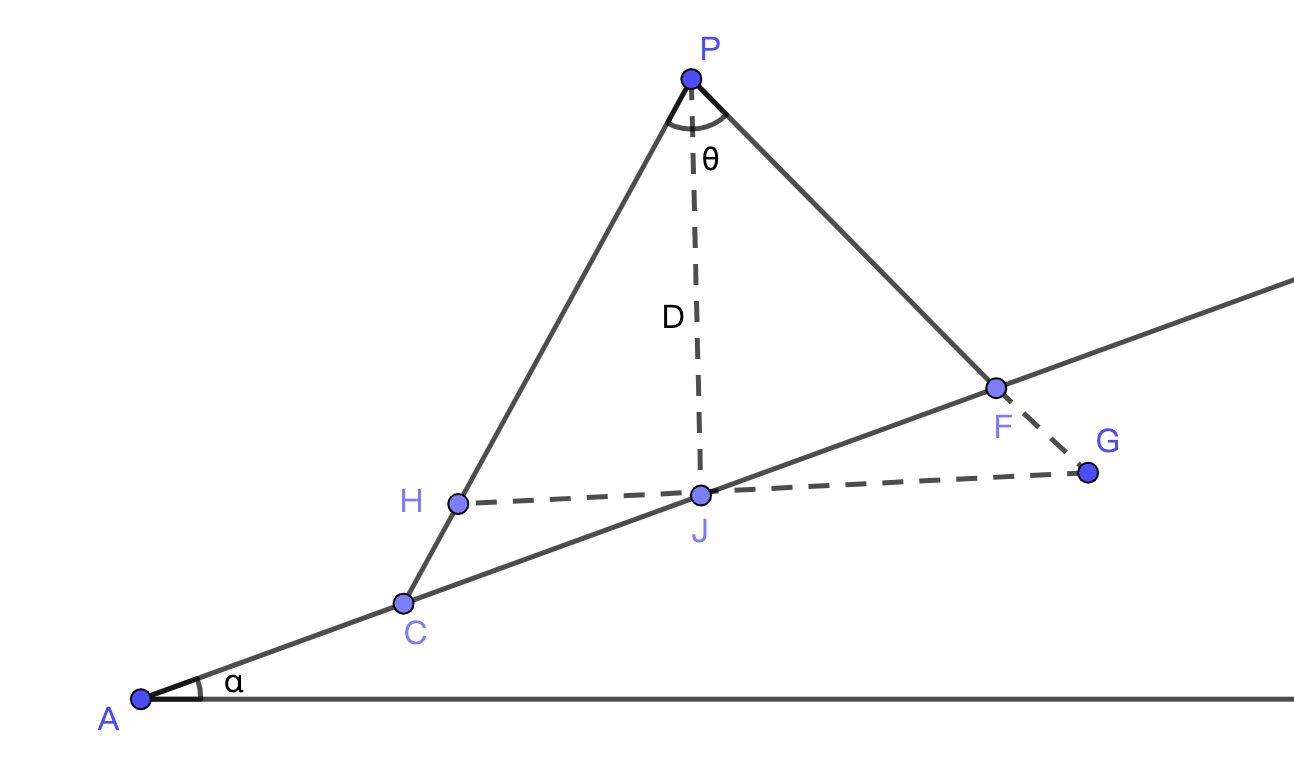
\includegraphics[width=.6\textwidth]{plot1-1}
    \caption{坡面情况下多波束测深初始位置的示意图}
    \label{fig:plot1-1}
\end{figure}

充分利用图形的几何特性,我们过波束张角$\angle CPF$的平分线$PJ$与坡面的交点$J$点作水平线,交波束$PC$和$PF$于$H$点和$G$点。分别在在$\Delta CHJ$和$\Delta GFJ$中由正弦定理得:
\begin{equation}
\frac{\sin\angle HCJ}{HJ} = \frac{\sin\angle CHJ}{CJ}
\label{eq:eq1-1}
\end{equation}

\begin{equation}
\frac{\sin\angle GFJ}{GJ} = \frac{\sin\angle FGJ}{FJ}
\label{eq:eq1-2}
\end{equation}

不难发现
\begin{equation}
HJ = JG = D \tan\frac{\theta}{2}
\label{eq:eq1-3}
\end{equation}
并且有角度关系
\begin{equation}
\angle FGJ = \frac{\pi}{2}-\frac{\theta}{2}  \qquad \angle CHJ = \frac{\pi}{2}+\frac{\theta}{2}
\label{eq:eq1-4}
\end{equation}

\begin{equation}
\angle FGJ = \frac{\pi}{2}+\frac{\theta}{2}-\alpha \qquad \angle HCJ = \frac{\pi}{2}-\frac{\theta}{2}-\alpha
\label{eq:eq1-5}
\end{equation}

联立上述各式,解得
\begin{equation}
CJ= \frac{D \sin \frac{\theta}{2}}{cos(\frac{\theta}{2} + \alpha)} \qquad JF= \frac{D \sin \frac{\theta}{2}}{cos(\frac{\theta}{2} - \alpha)}
\label{eq:eq1-6}
\end{equation}

\begin{figure}[!h]
    \centering
    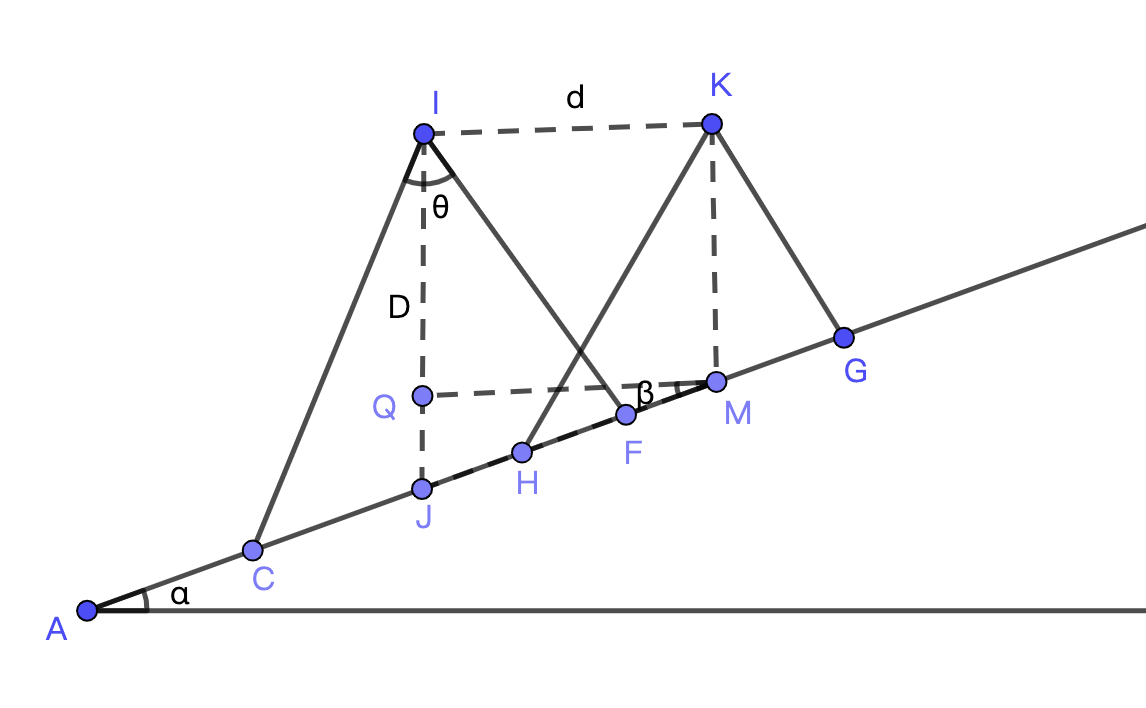
\includegraphics[width=.6\textwidth]{plot1-2}
    \caption{海底存在坡面情况下多波束测深动态变化的示意图}
    \label{fig:plot1-2}
\end{figure}

当测量船如\textbf{图2}沿着侧线移动时,两条波束与坡面相交形成的三角形总是相似的。以本图所显示的初末位置为例,有
\begin{equation}
\Delta CPF \sim \Delta HKG
\label{eq:eq1-7}
\end{equation}

过$M$点向$PJ$作垂线,观察得到
\begin{equation}
KM = D - d \tan \beta
\label{eq:eq1-8}
\end{equation}
且显然有
\begin{equation}\alpha = \beta
\label{eq:eq1-9}
\end{equation}
运用三角形相似比,得到
\begin{equation}
GM = \frac{KM}{PJ} FJ \qquad MH = \frac{KM}{PJ} CJ
\label{eq:eq1-10}
\end{equation}

因此得到
\begin{equation}
HF = JF+MH-MJ = \frac{D \sin \frac{\theta}{2}}{\cos(\frac{\theta}{2}-\alpha)} + \frac{(D-d\tan \alpha) \sin \frac{\theta}{2}}{\cos(\frac{\theta}{2}+\alpha)}-\frac{d}{\cos \alpha}
\label{eq:eq1-10}
\end{equation}

在测线相互平行且海底地形平坦的情况下,相邻条带之间的重叠率定义为 $\eta = 1−\frac{d}{W}$。其中$d$ 为相邻两条测线的间距,$W$ 为条带的覆盖宽度。在有坡度的情况下,由于测线所包含的覆盖线(即$CF$,$HG$)时时发生变化,该定义不再适用。

因此我们定义,在有坡度的情况下,条带的重叠率$\eta$为\textbf{该测线所包含的覆盖线与前一条侧线所包含的覆盖线的比值}。在\textbf{图2}中可以具体表示为:
\begin{equation}
\eta = \frac{HF}{CF}
\label{eq:eq1-11}
\end{equation}

联立上述各式,得到最终结果
\begin{equation}
\eta = 1 - \frac{d}{2D}(\frac{1}{\tan \frac{\theta}{2}}+\tan \alpha)
\label{eq:eq1-12}
\end{equation}

\subsubsection{共点相似三角形解法}

结合\textbf{图3},还有另一种推导方法:
\begin{figure}[!h]
    \centering
    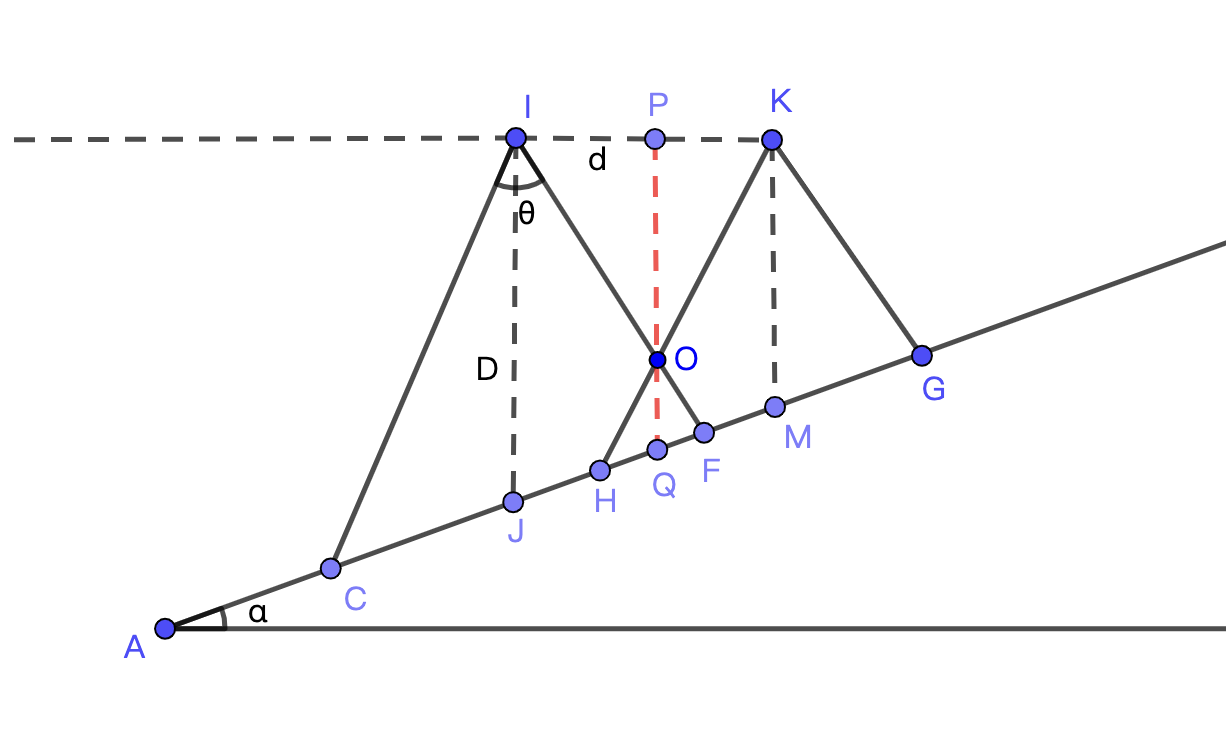
\includegraphics[width=.6\textwidth]{plot3-1}
    \caption{另一种推导方法}
    \label{fig:plot1-1}
\end{figure}
由于平行关系,不难发现
\begin{equation}
\angle IOP = \angle POR = \frac{\theta}{2}
\label{eq:eq1-13}
\end{equation}
因此$P$是$IR$中点,梯形$KMJI$的中位线
\begin{equation}
PQ = \frac{1}{2}(2D-d\tan\alpha)
\label{eq:eq1-14}
\end{equation}
以及有
\begin{equation}
OQ = PQ - PO = D - \frac{1}{2}d\tan\alpha-\frac{d}{2\tan\frac{\theta}{2}} 
\label{eq:eq1-15}
\end{equation}
以$F$为顶点的几组平行相似三角形给出关系:
\begin{equation}
\frac{OQ}{IJ}= \frac{OF}{IF} = \frac{HF}{AF} = \eta
\label{eq:eq1-16}
\end{equation}

联立同样得到 
\begin{equation}
\eta = 1 - \frac{d}{2D}(\frac{1}{\tan \frac{\theta}{2}}+\tan \alpha)
\label{eq:eq1-12}
\end{equation}

两种解法得到的结果相同,表明表达式准确、可信。我们观察发现,覆盖率$\eta$只是移动间距$d$,深度$D$,以及张角$\theta$和坡角$\alpha$的函数。该模型定量反映了覆盖率的影响因素,为下面更加具体、实际的问题奠定基础。

\subsubsection{填充表格}
基于这样的模型,我们用代码填充对应表格,得到填充结果如\textbf{表1}:
\begin{table}[!h]
\centering
\caption{问题 1 的计算结果}
\label{tab:my-table}
\resizebox{\columnwidth}{!}{%
\begin{tabular}{|c|c|c|c|c|c|c|c|c|c|}
\hline
测线距中心点处的距离/m  & -800   & -600   & -400  & -200  & 0     & 200   & 400   & 600    & 800    \\ \hline
海水深度/m        & 90.95  & 85.71  & 80.47 & 75.24 & 70    & 64.76 & 59.53 & 54.29  & 49.05  \\ \hline
覆盖宽度/m        & 131.78 & 112.12 & 92.46 & 72.81 & 53.15 & 33.49 & 13.84 & -5.82  & -25.47 \\ \hline
与前一条测线的重叠率/\% & ——     & 29.59  & 25.00 & 19.78 & 13.78 & 6.81  & -1.39 & -11.17 & -23.04 \\ \hline
\end{tabular}%
}
\end{table}
\subsection{【问题2】测线方向与坡面法向水平投影夹角不为直角时的数学模型}
\subsubsection{转化和化归法}
结合化归的思想,我们倾向于将问题2中的情形(如\textbf{图4})转化为问题1。
\begin{figure}[!h]
    \centering
    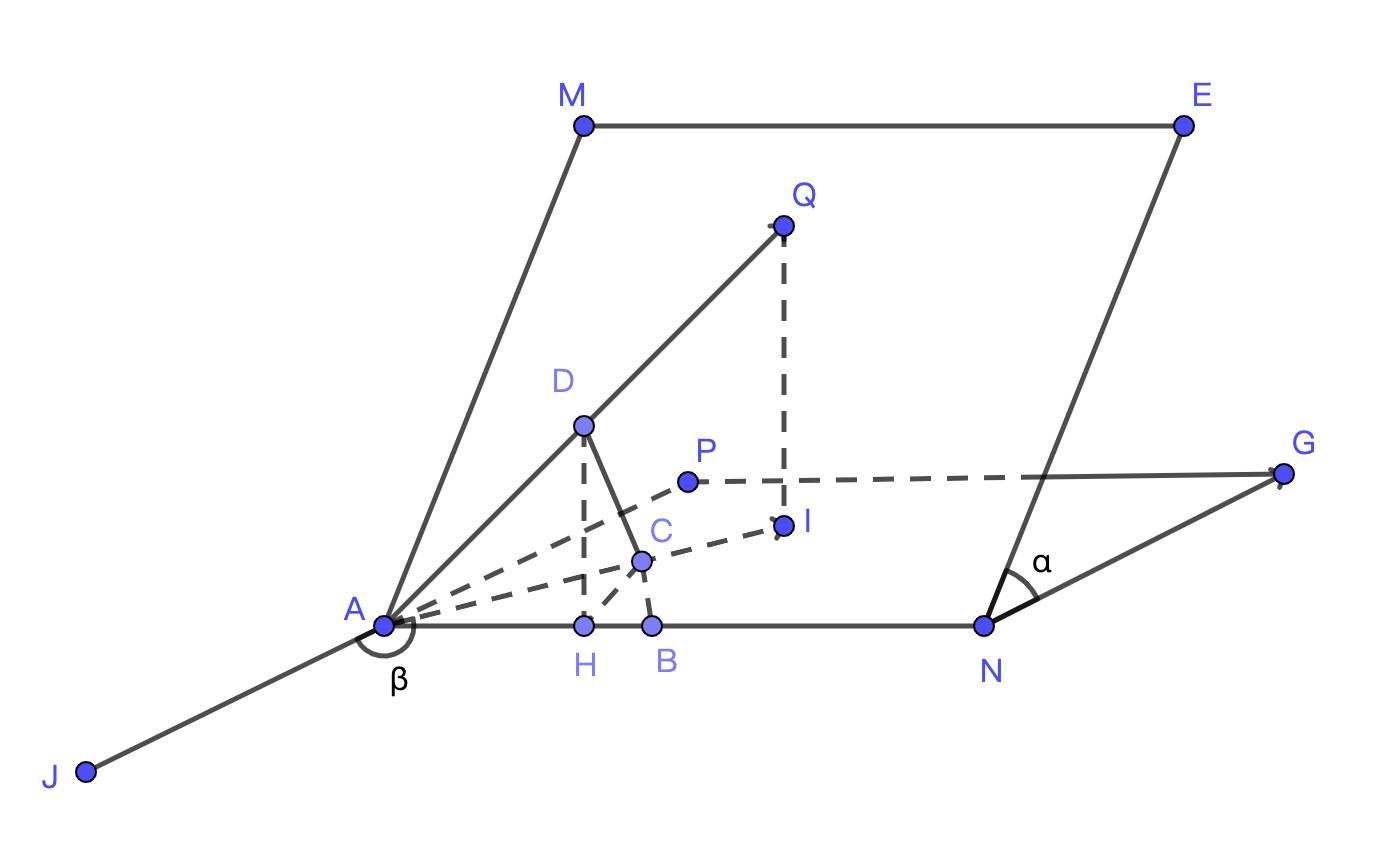
\includegraphics[width=.6\textwidth]{plot2}
    \caption{问题2中的情形}
    \label{fig:result1}
\end{figure}
据分析,问题1中测线方向与海底坡面的法向在水平面上投影的夹角为$\beta = \frac{\pi}{2}$。
推广到一般的角度$\beta$,我们沿着侧线重新建立如图所示的坡面$\angle DBC$(记作$\alpha_0$),以达到和问题1类似的效果。不难表示出坡度角
\begin{equation}
\tan \alpha_0 = \frac{DC}{BC}
\label{eq:eq2-1}
\end{equation}

我们引入辅助平面$CDH$ $\parallel$ 平面$NEG$:在$\Delta CDH$中,
\begin{equation}
CD = CH\tan\alpha
\label{eq:eq2-2}
\end{equation}
过$C$点作$AI$的垂线,交$AN$于$B$点:在$\Delta CHB$中,
\begin{equation}
CH = BC \cos\angle CAB = \cos(\beta-\frac{\pi}{2})
\label{eq:eq2-3}
\end{equation}
联立上述各式,有
\begin{equation}
\alpha_0 = \arctan (\sin\beta \tan\alpha)
\label{eq:eq2-4}
\end{equation}

作为对问题1中$\eta = 1 - \frac{d}{2D}(\frac{1}{\tan \frac{\theta}{2}}+\tan \alpha)$的推广,我们有
\begin{equation}
\eta = 1 - \frac{d}{2D}(\frac{1}{\tan \frac{\theta}{2}}+\sin\beta \tan\alpha)
\label{q:eq2-4}
\end{equation}

\subsubsection{填充表格}
基于这样的模型,我们用代码填充对应表格,得到填充结果如\textbf{表2}:
\begin{table}[!h]
\centering
\caption{问题2的计算结果}
\label{tab:my-table}
\begin{tabular}{|lc|cccccccc|}
\hline
\multicolumn{2}{|l|}{\multirow{2}{*}{覆盖宽度/m}}         & \multicolumn{8}{l|}{测量船距海域中心点处的距离/海里}                                                                                                                                                            \\ \cline{3-10} 
\multicolumn{2}{|l|}{}                                & \multicolumn{1}{c|}{0}   & \multicolumn{1}{c|}{0.3} & \multicolumn{1}{c|}{0.6} & \multicolumn{1}{c|}{0.9} & \multicolumn{1}{c|}{1.2} & \multicolumn{1}{c|}{1.5} & \multicolumn{1}{c|}{1.8} & 2.1 \\ \hline
\multicolumn{1}{|l|}{\multirow{8}{*}{测线方向夹角/°}} & 0   & \multicolumn{1}{c|}{416} & \multicolumn{1}{c|}{466} & \multicolumn{1}{c|}{516} & \multicolumn{1}{c|}{567} & \multicolumn{1}{c|}{617} & \multicolumn{1}{c|}{668} & \multicolumn{1}{c|}{718} & 768 \\ \cline{2-10} 
\multicolumn{1}{|l|}{}                          & 45  & \multicolumn{1}{c|}{416} & \multicolumn{1}{c|}{452} & \multicolumn{1}{c|}{488} & \multicolumn{1}{c|}{523} & \multicolumn{1}{c|}{559} & \multicolumn{1}{c|}{595} & \multicolumn{1}{c|}{630} & 666 \\ \cline{2-10} 
\multicolumn{1}{|l|}{}                          & 90  & \multicolumn{1}{c|}{417} & \multicolumn{1}{c|}{417} & \multicolumn{1}{c|}{417} & \multicolumn{1}{c|}{417} & \multicolumn{1}{c|}{417} & \multicolumn{1}{c|}{417} & \multicolumn{1}{c|}{417} & 417 \\ \cline{2-10} 
\multicolumn{1}{|l|}{}                          & 135 & \multicolumn{1}{c|}{416} & \multicolumn{1}{c|}{381} & \multicolumn{1}{c|}{345} & \multicolumn{1}{c|}{309} & \multicolumn{1}{c|}{273} & \multicolumn{1}{c|}{238} & \multicolumn{1}{c|}{202} & 166 \\ \cline{2-10} 
\multicolumn{1}{|l|}{}                          & 180 & \multicolumn{1}{c|}{416} & \multicolumn{1}{c|}{365} & \multicolumn{1}{c|}{315} & \multicolumn{1}{c|}{264} & \multicolumn{1}{c|}{214} & \multicolumn{1}{c|}{164} & \multicolumn{1}{c|}{113} & 63  \\ \cline{2-10} 
\multicolumn{1}{|l|}{}                          & 225 & \multicolumn{1}{c|}{416} & \multicolumn{1}{c|}{381} & \multicolumn{1}{c|}{345} & \multicolumn{1}{c|}{309} & \multicolumn{1}{c|}{273} & \multicolumn{1}{c|}{238} & \multicolumn{1}{c|}{202} & 166 \\ \cline{2-10} 
\multicolumn{1}{|l|}{}                          & 270 & \multicolumn{1}{c|}{417} & \multicolumn{1}{c|}{417} & \multicolumn{1}{c|}{417} & \multicolumn{1}{c|}{417} & \multicolumn{1}{c|}{417} & \multicolumn{1}{c|}{417} & \multicolumn{1}{c|}{417} & 417 \\ \cline{2-10} 
\multicolumn{1}{|l|}{}                          & 315 & \multicolumn{1}{c|}{416} & \multicolumn{1}{c|}{452} & \multicolumn{1}{c|}{488} & \multicolumn{1}{c|}{523} & \multicolumn{1}{c|}{559} & \multicolumn{1}{c|}{595} & \multicolumn{1}{c|}{630} & 666 \\ \hline
\end{tabular}
\end{table}



\newpage
\subsection{【问题3】矩形海域测线规划方案}
\subsubsection{测线方向的讨论}
从模型的简洁性考虑,我们不妨规划一组平行于矩形边界的测线组。我们使用动态规划的思路,迭代的算法,从边界情况开始考虑,直至所有的区域已经被全部覆盖。
\begin{figure}[!h]
    \centering
    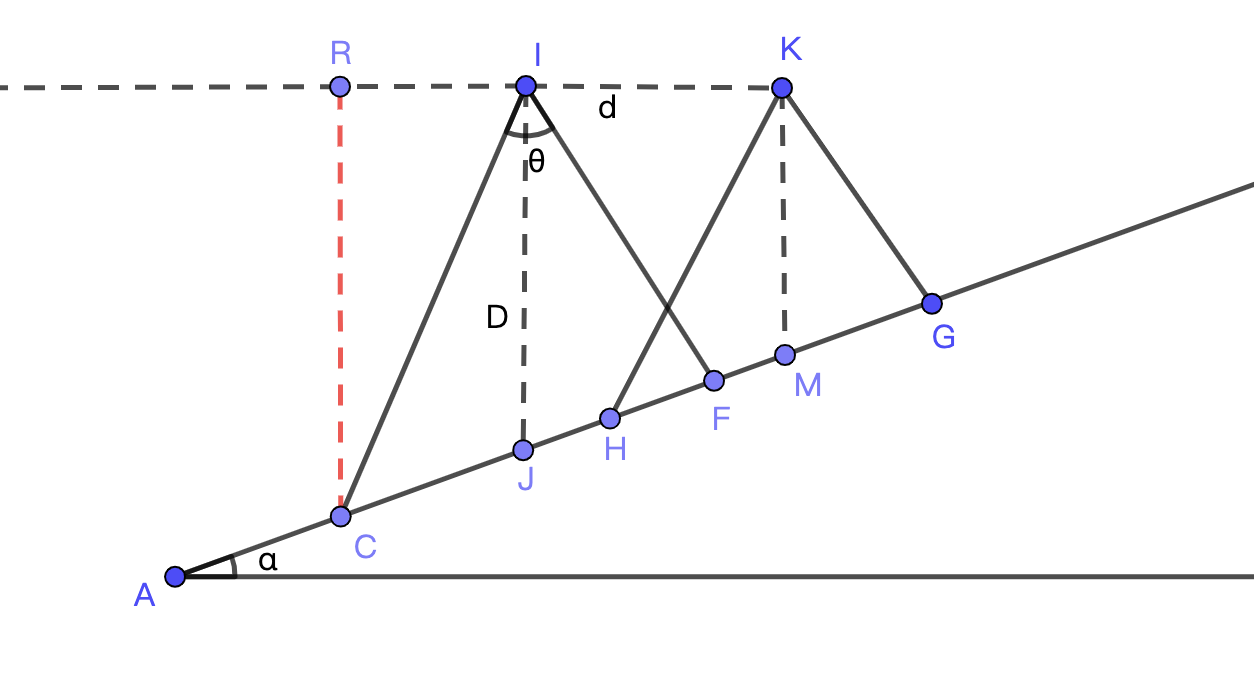
\includegraphics[width=.6\textwidth]{plot3-2}
    \caption{边界情况示意图}
    \label{fig:result1}
\end{figure}
\begin{figure}
    \centering
    \begin{minipage}[c]{0.4\textwidth}
        \centering
        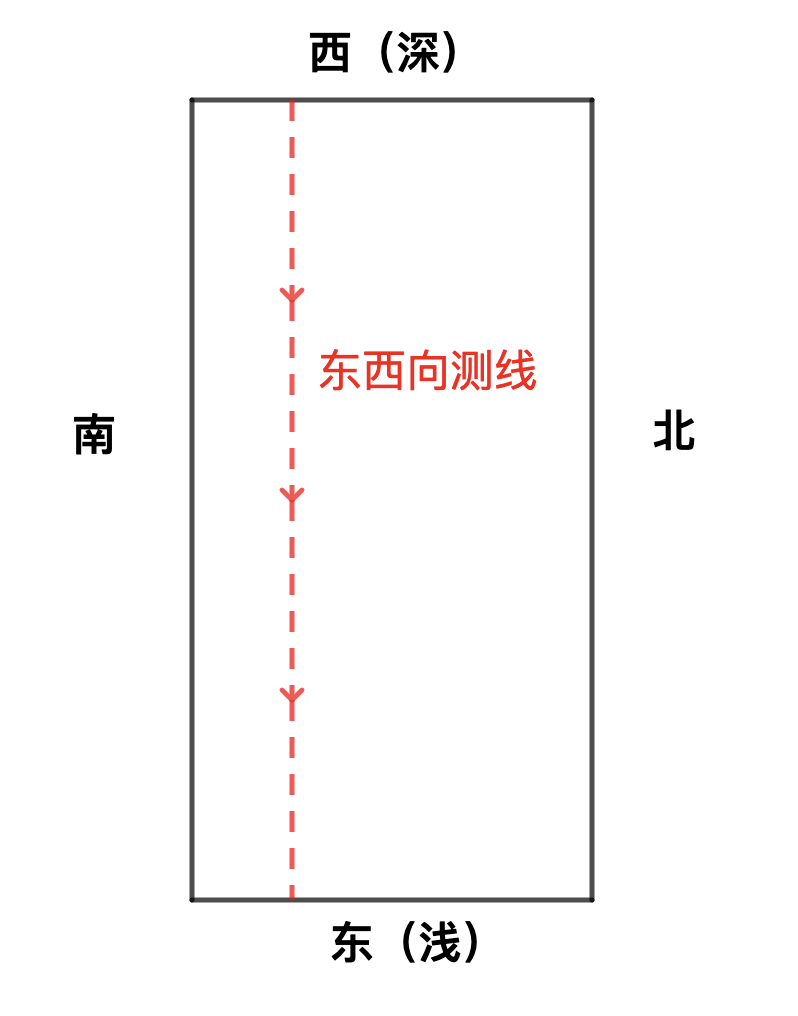
\includegraphics[height=0.3\textheight]{plot3-4}
        \subcaption{测线示意图}
    \end{minipage}
    \begin{minipage}[c]{0.4\textwidth}
        \centering
        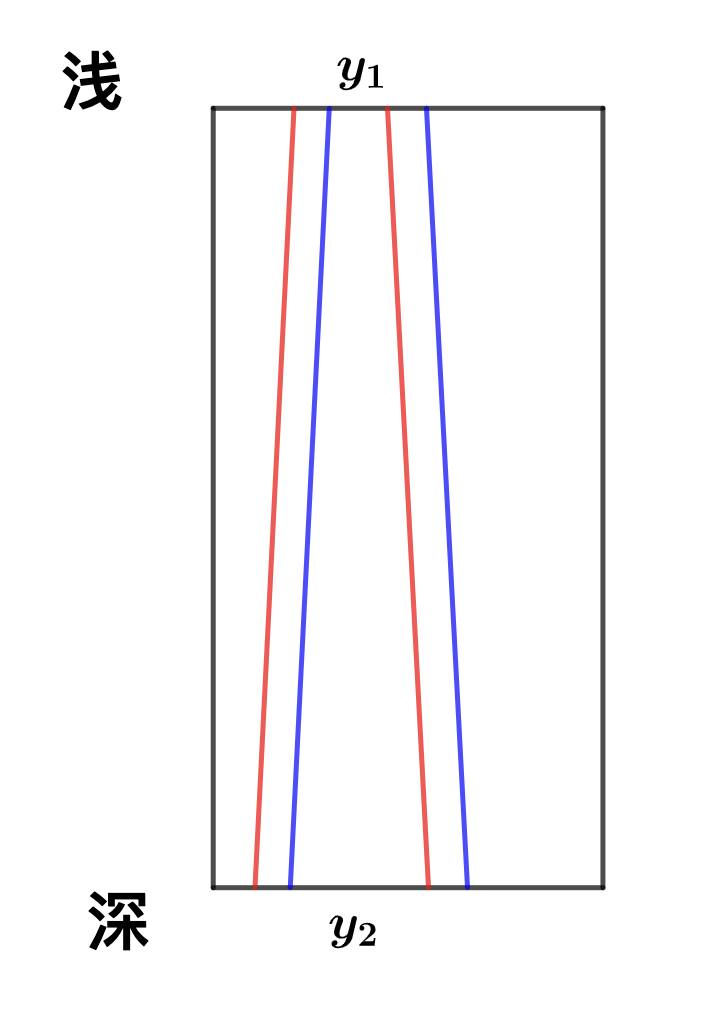
\includegraphics[height=0.3\textheight]{plot3-5}
        \subcaption{扫描在海床上的投影示意图}
    \end{minipage}
    \begin{minipage}[c]{0.4\textwidth}
        \centering
        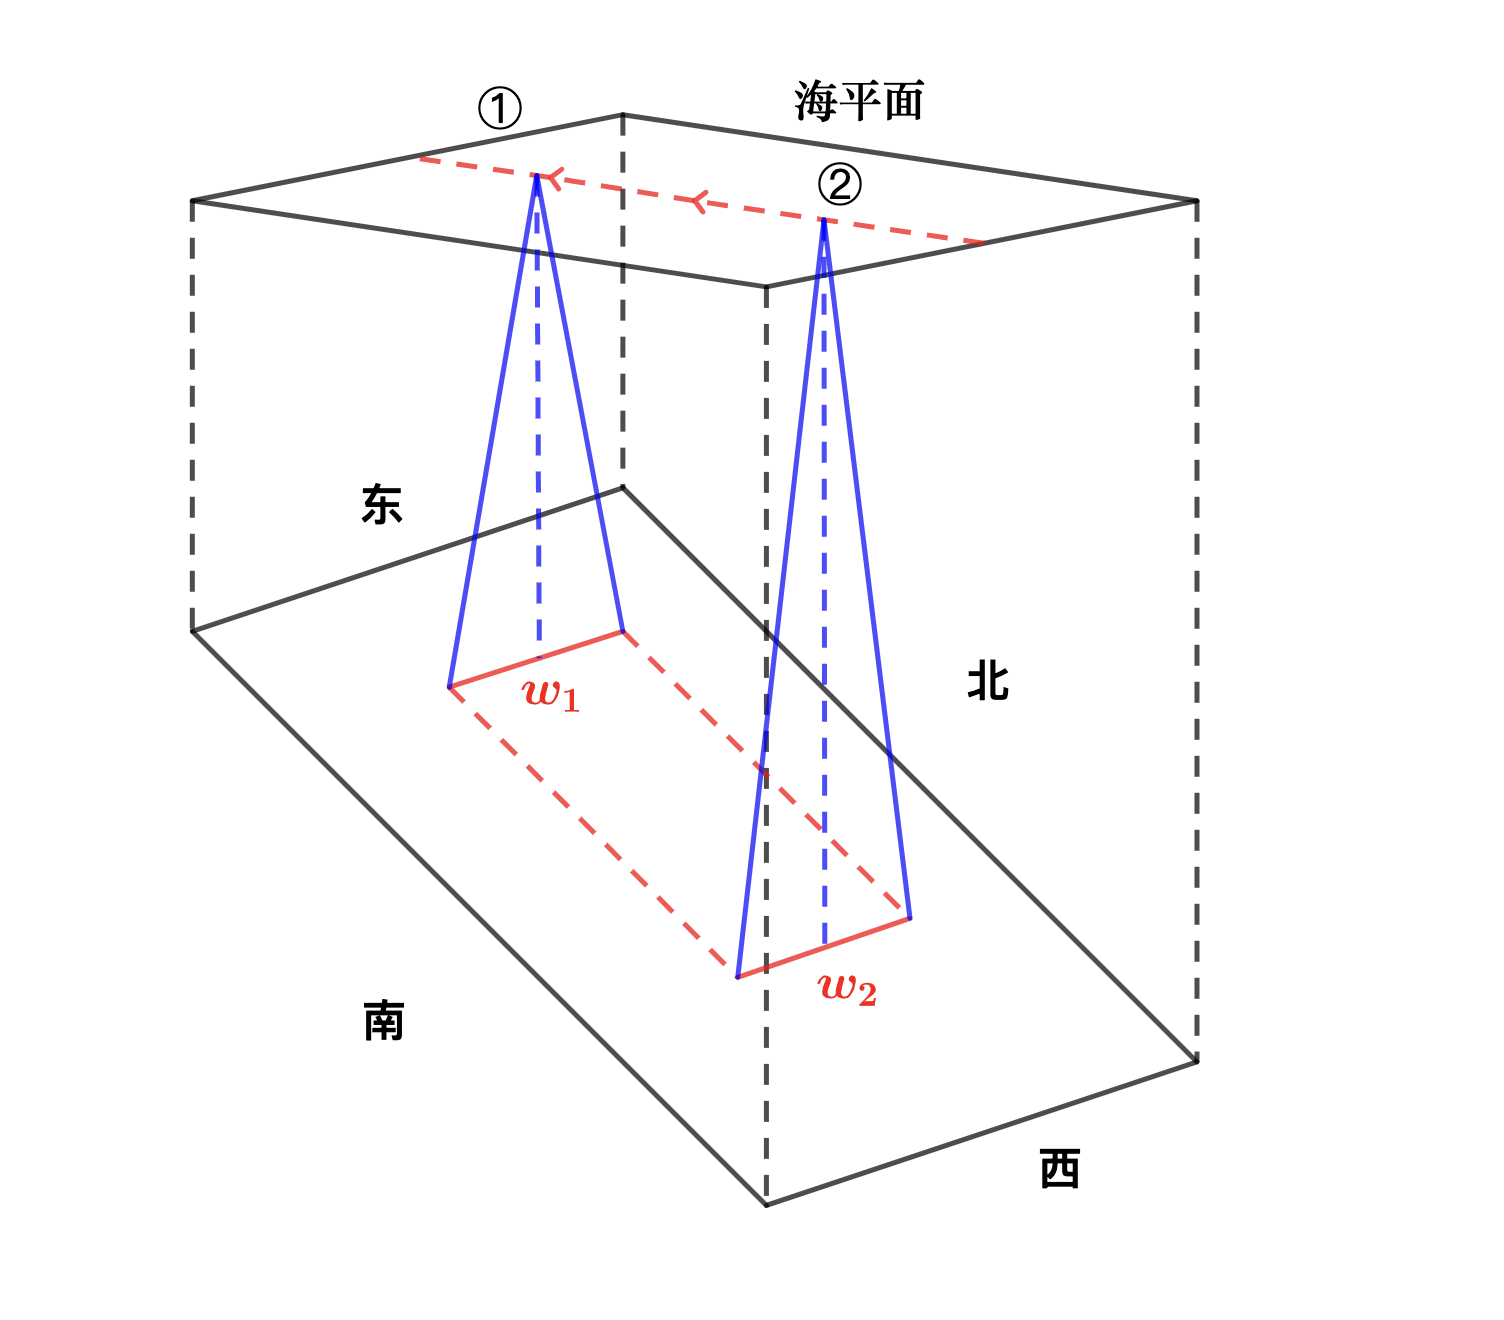
\includegraphics[height=0.3\textheight]{plot3-3}
        \subcaption{扫描立体示意图}
    \end{minipage}
    \caption{东西向测线示意图}
\end{figure}
现在我们讨论应该是采用东西向的测线组,还是南北向的测线组。我们首先讨论东西向侧线(\textbf{图6(a)})的情况。由于每一次波束的扫描面和海底的交线到海平面的距离不同(即$w_1<w_2$,如\textbf{图6(c)}),在海床上将扫描出一个梯形的形状。

我们以海底面法向量的方向俯视波束扫描在海床上的图形投影,如\textbf{图6(b)}所示,红色为初始扫描的投影,蓝色为移动后的扫描投影。我们发现,总有上宽度$y_1<y_2$。这对在有大约100米东西落差的海床上实现$y_1 >0.1$,$y_2<0.2$的要求明显较为麻烦。结合测绘力求精简实际需求,我们不再考虑东西向的测线方案。

但是南北向的测线由于每一次波束的扫描面和海底的交线到海平面的距离总是一致,所以抛却了上述困难。针对图形特点,我们充分利用动态规划的方案,用迭代的算法进行路线规划。

\subsubsection{测线顺序的讨论和具体计算}
下面我们将具体探讨对于南北向测线从西侧和从东侧开始的情况。


从\textbf{图5}可以看到,$C$点是覆盖面可以扫到的最左侧边界。如果从西侧开始,对于第1条侧线,我们将过$C$点垂直于纸面的直线与西侧边界重合,构建基本的几何图形结构,可以得到$I$点的位置,过$I$点垂直于纸面的直线即为第1条侧线。根据既定的覆盖率,我们又可以推到第2条测线所在位置$K$点……以此类推,直到第$n$条侧线时,覆盖面可以扫到的最右侧边界$G$点第一次超越东侧边界为止。



我们约定,把第一条测线记作第$0$次,我们约定第$i$次测线到垂直下端坡面的距离为$D_i$,第$i$次与第$i+1$次的测线间隔为$d_i$,第$i$次的线段长度分别为$CJ_i$和$MG_i$。

最开始的边界情况是:$CJ_0 \sin\alpha + D_0 = h_{west}$,可以得到$D_0$的值。
对于每一个$i>1$的情形,总有$D_i = D_{i-1}-d_{i-1}\tan \alpha$ 来算出新的$D_i$。直到第一次满足$MG_i +\sum_{i=1}^{n}d_i \geq L$,跳出循环。这一过程用伪代码可以表示为:

\begin{algorithm}
\caption{Compute \(D_i\)}
\begin{algorithmic}[1]
\REQUIRE \(CJ_0, \alpha, h_{\text{west}}, L, \{d_i\}_{i=1}^{n}\)
\ENSURE \(D_i\)
\STATE \(D_0 \leftarrow h_{\text{west}} - CJ_0 \sin\alpha\)
\STATE \text{sum\_distance} \( \leftarrow 0\)
\FOR{\(i = 1\) \TO \(n\)}
    \STATE \(D_i \leftarrow D_{i-1} - d_{i-1} \tan\alpha\)
    \STATE \text{sum\_distance} \( \leftarrow \text{sum\_distance} + d_i\)
    \IF{\(MG_i + \text{sum\_distance} \geq L\)}
        \STATE \text{break}
    \ENDIF
\ENDFOR
\end{algorithmic}
\end{algorithm}


在第一问中我们得到
\begin{equation}
\eta = 1 - \frac{d}{2D}(\frac{1}{\tan \frac{\theta}{2}}+\tan\alpha)
\label{q:eq3-1}
\end{equation}
我们还得到长度参数(分别与对应的$D$对应)

\begin{equation}
CJ= \frac{D \sin \frac{\theta}{2}}{cos(\frac{\theta}{2} - \alpha)} \qquad MG= \frac{D \sin \frac{\theta}{2}}{cos(\frac{\theta}{2} - \alpha)}
\label{q:eq3-2}
\end{equation}

至于具体覆盖率 $\eta$的取值,过大的覆盖率必然导致测线条数太多造成冗杂,过小的覆盖率又会导致某些地段不能完全测准。结合实际情况和实践经验,考虑设定 $\eta = 0.1$为宜。

如果从东侧开始,则与上述过程完全类似。由于不一定能够最后一次的边界情况可能取不到等号,所以可能会覆盖一个实际上稍大的区域,因此从西向东和从东向西理应不完全一致,但是不应该相差过大。
\subsubsection{测线方案结果及可视化}
\begin{figure}
    \centering
    \begin{minipage}[c]{0.3\textwidth}
        \centering
        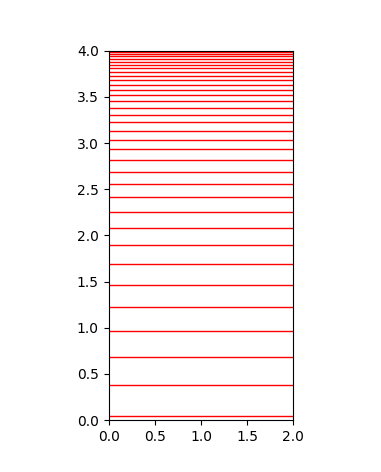
\includegraphics[height=0.2\textheight]{plot3-2-1}
        \subcaption{从东向西示意图}
    \end{minipage}
    \begin{minipage}[c]{0.3\textwidth}
        \centering
        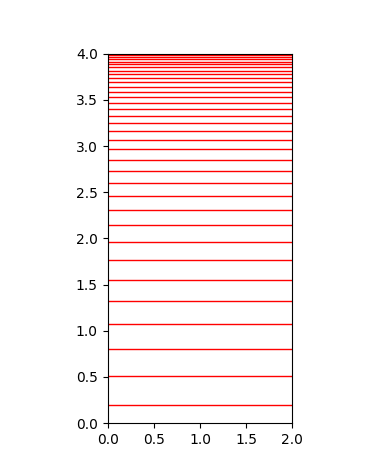
\includegraphics[height=0.2\textheight]{plot3-2-2}
        \subcaption{从西到东示意图}
    \end{minipage}
    \begin{minipage}[c]{0.3\textwidth}
        \centering
        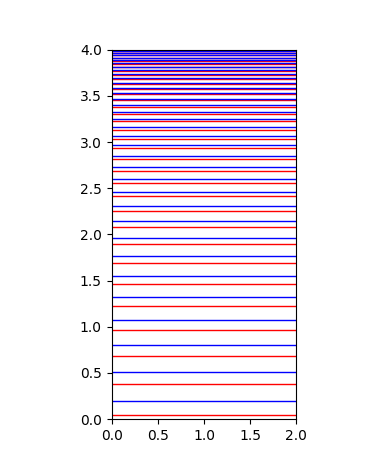
\includegraphics[height=0.2\textheight]{plot3-3-3}
        \subcaption{总览示意图}
    \end{minipage}
    \caption{测线规划示意图}
\end{figure}
最终我们得到了测线规划示意图,分别可见\textbf{图7(a)}、\textbf{图7(b)}和\textbf{图7(c)}。具体参数可以通过\textbf{附录B}代码“具体参数”获得。概括来看,从东向西一共有 34 条测线,总路程为 125936 米(68 海里);从西向东一共有 34 条测线,总路程为 125936 米(68 海里)。结果几乎一致,印证了我们的设想。


\subsection{【问题4】实际海域测线应用方案}
根据给出的数据集,经过简单的数据清理我们作出海底平面的热力图(\textbf{图8(a)})和3D图(\textbf{图8(b)}))以供初步观察:
\begin{figure}[htbp]
    \centering
    \begin{minipage}{0.45\textwidth}
        \centering
        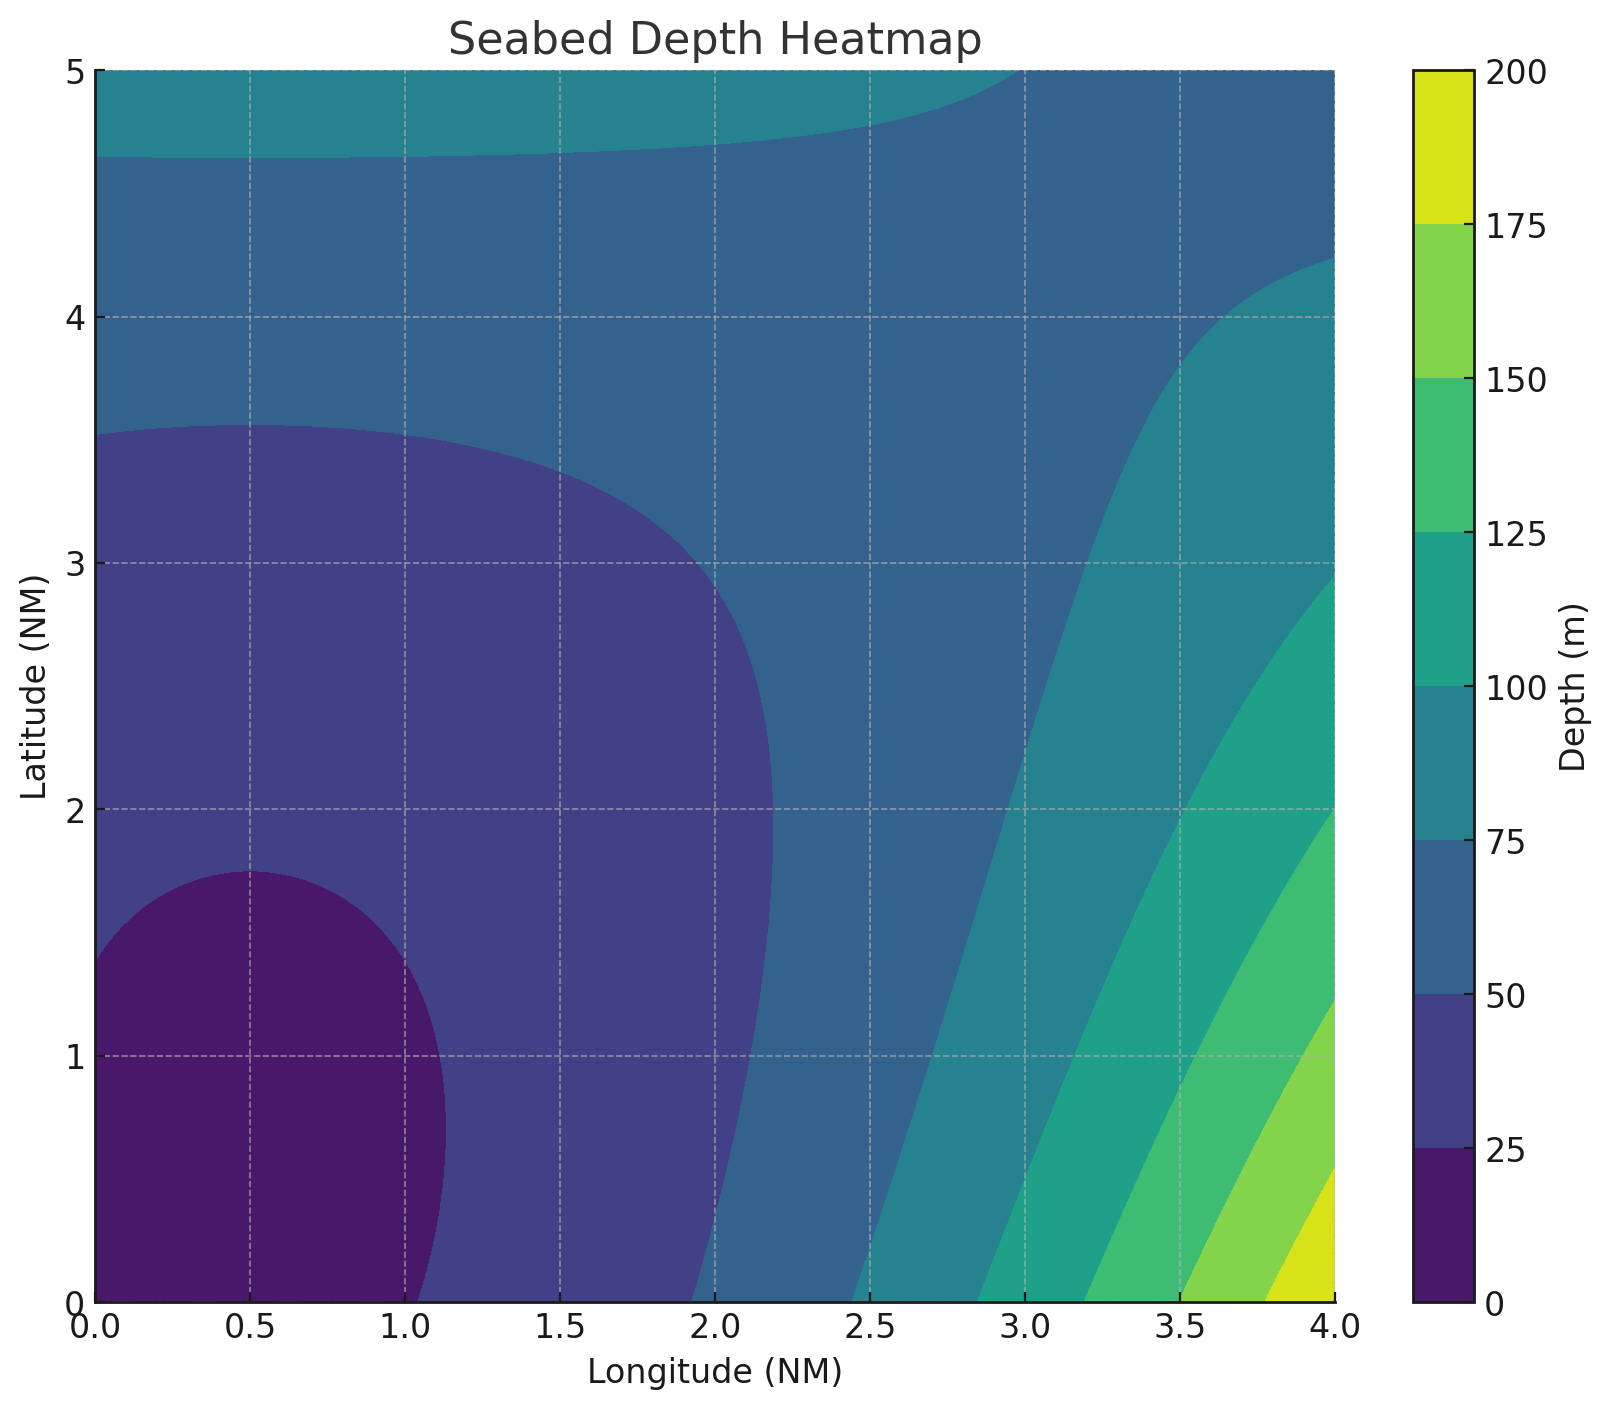
\includegraphics[width=\linewidth]{plot4-1}
        \subcaption{实际海底热力图}
    \end{minipage}
    \hfill
    \begin{minipage}{0.45\textwidth}
        \centering
        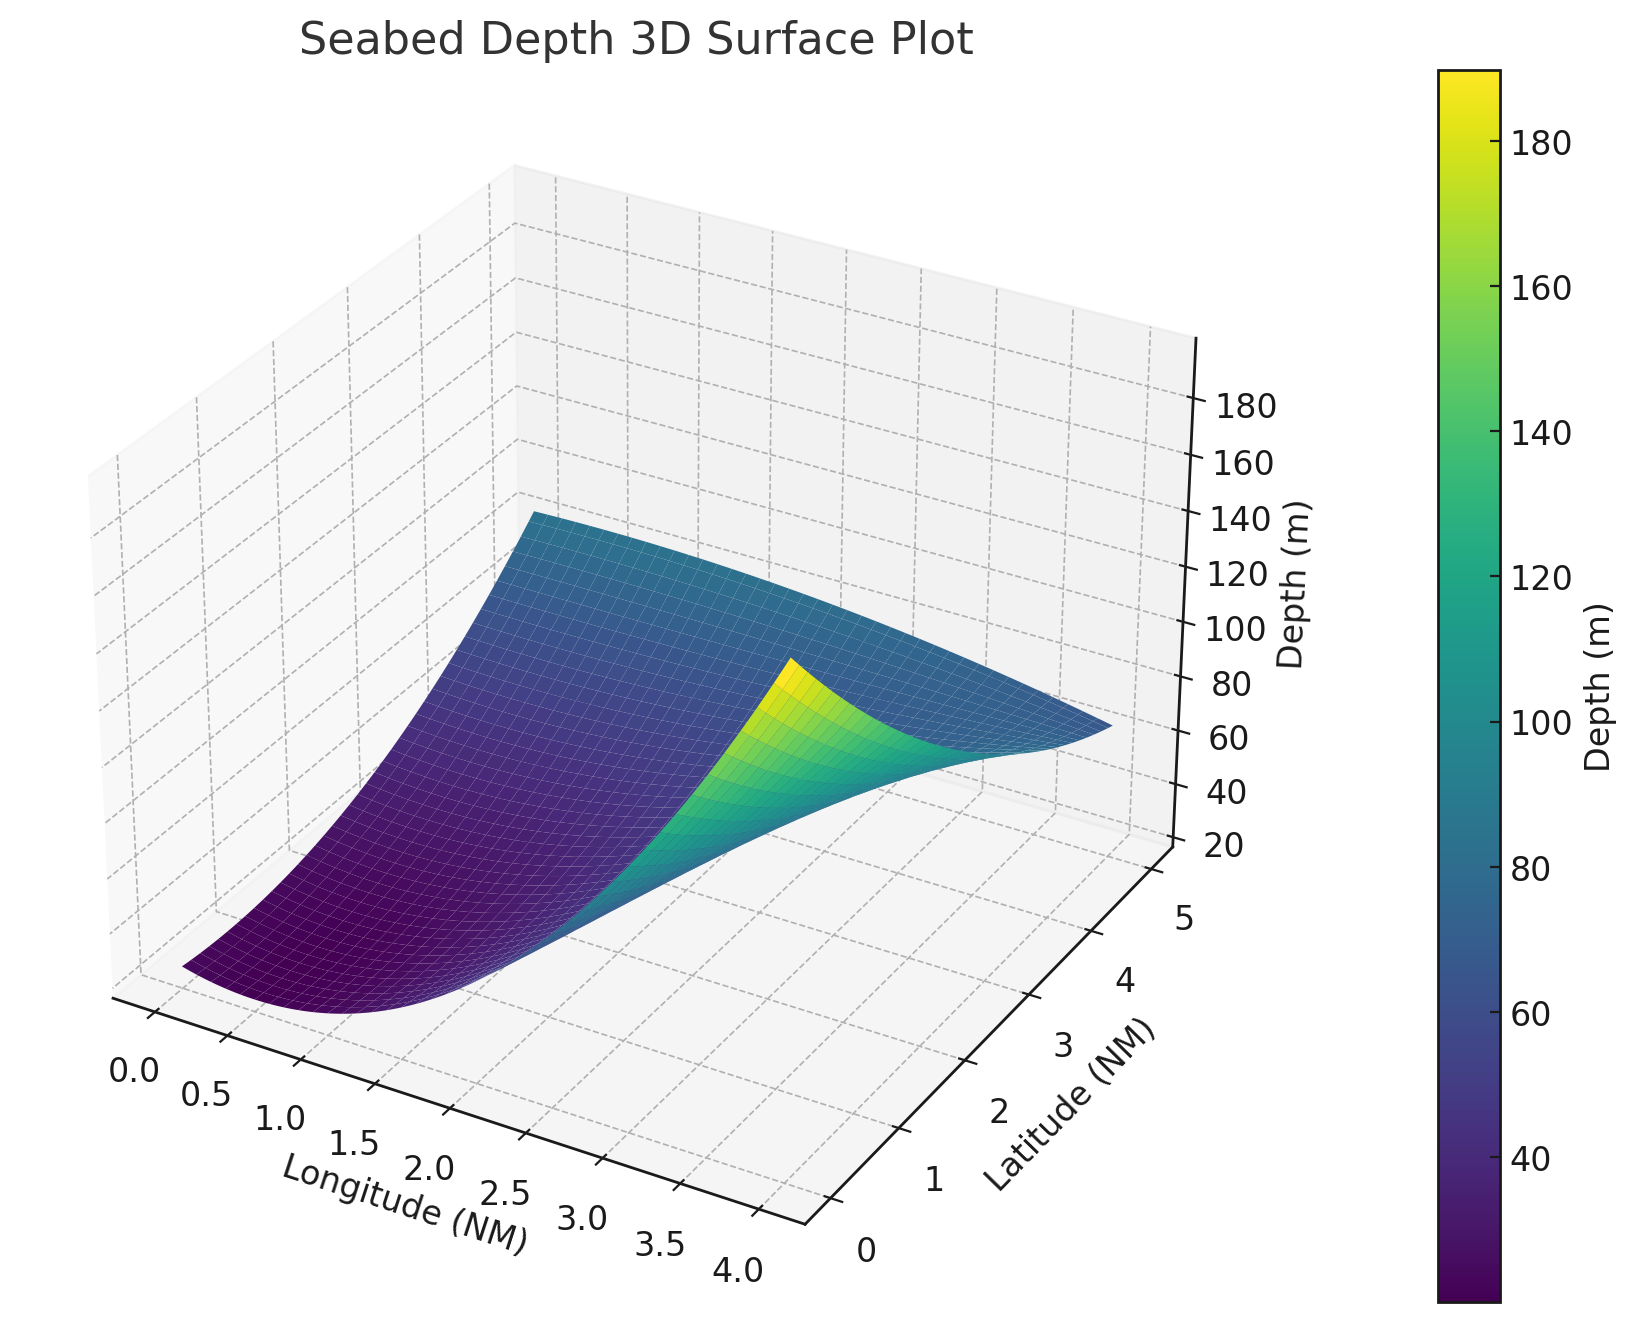
\includegraphics[width=\linewidth]{plot4-2}
        \subcaption{实际海底3D图}
    \end{minipage}
    \caption{实际海底平面示意图}
\end{figure}


\subsubsection{定量分析结果}
根据对热力图的观察、结合具体实际情况,我们选择将海底面分为四个部分,每个部分进行平面的线性回归拟合,最终化归为问题3中的情形进行解决。
\begin{figure}[!h]
    \centering
    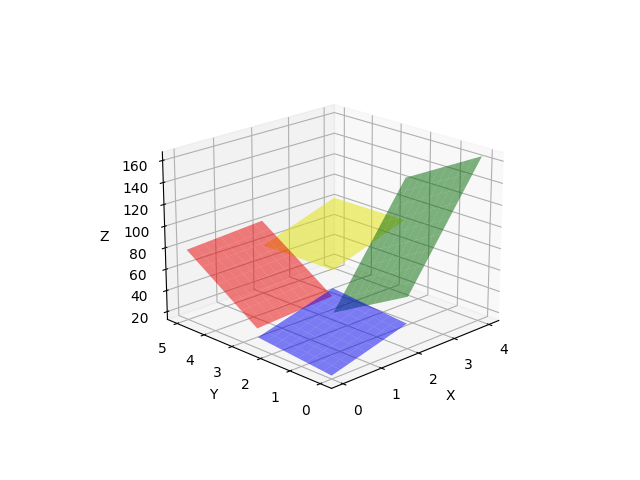
\includegraphics[width=.9\textwidth]{plot4-3}
    \caption{线性回归拟合平面}
    \label{fig:plot4-3}
\end{figure}
\FloatBarrier
对于每个平面,我们假设向量表达式为
\begin{equation}
\Vec{y} = X \Vec{w} + \vec{\epsilon}
\end{equation}
我们需要
\begin{equation}
\mathop{\min}_{w} \, \epsilon^T\epsilon
\end{equation}

通过计算每个样本点和拟合平面之间都存在的误差,我们选取总误差最小的那个平面为目标平面,运用最小二乘法的思想,最终得到如\textbf{图9}所示的结果,然后对四个区域分别进行计算处理。

至于覆盖率,我们的算法是:对于数据集中的每一个点,首先找到与之最近的一对测线,并分别计算该点到这对测线垂直距离与海平面的夹角,如果都大于$\frac{\theta}{2}$,就不可以测得。最终积分求到遗漏的面积,得出覆盖率。

根据代码呈现的结果(可视化可见\textbf{图10}),我们完成了测线的规划。
\begin{figure}[!h]
    \centering
    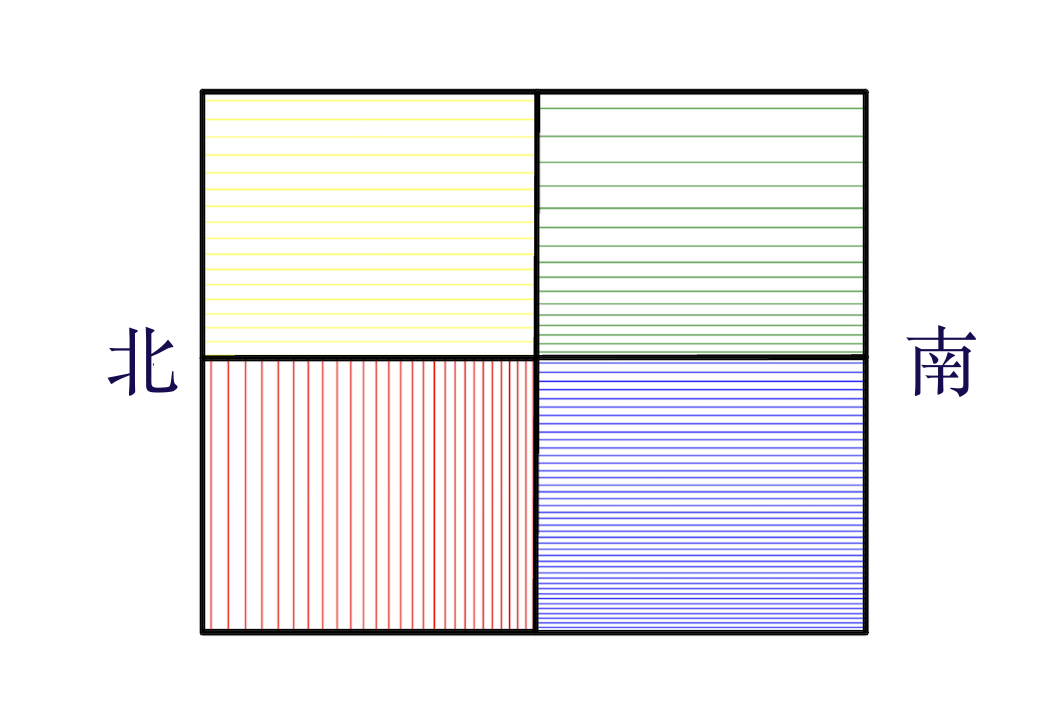
\includegraphics[width=.7\textwidth]{plot4-5}
    \caption{实际海域规划路线图}
    \label{fig:plot4-3}
\end{figure}
蓝色部分一共有 43 条测线,总路程为107.5海里,遗漏率为11.50$\%$;绿色部分一共有 16 条测线,总路程为40.0 海里,遗漏率为 13.04$\%$;红色部分一共有 28 条测线,总路程为56 海里,遗漏率为 10.79$\%$;黄色部分一共有 17 条测线,总路程为42.5 海里,遗漏率为 2.91$\%$。
\subsubsection{定性分析探索}
\paragraph*{拉普拉斯算子的基本原理}
拉普拉斯算子(Laplace operator)的基本思路和原理是描述函数在三维空间中的空间变化。
它测量了函数在不同方向上的曲率和变化率,因此可以用于研究函数在空间中的平滑性、梯度、散度和二阶导数等性质。

它通常表示为 $\nabla^2$, 或者有时候也写成 $\Delta$。它是一个二阶偏微分算子,定义如下:
\[\nabla^2 = \frac{\partial^2 f}{\partial x^2} + \frac{\partial^2 f}{\partial y^2} + \frac{\partial^2 f}{\partial z^2} \]
在这个定义中,$f$ 是一个函数,它的输入是三维空间中的一个点,输出是一个实数。

同时,我们注意到,拉普拉斯算子用于描述函数在三维空间中的空间变化,它测量了函数在不同方向上的曲率和变化率,帮助我们理解函数如何在空间中变化;
同时,它还可以用于定义梯度和散度运算。梯度描述了函数的空间变化率,而散度描述了向量场的发散程度。

\paragraph*{拉普拉斯算子在本题的应用}
在前述测算中,我们对海域进行了平均分割并进行了线性回归拟合,然而,在实际操作中,存在更为精细的非均匀海域分割方法。
受到拉普拉斯算子的启发,我们在每个点处执行类似于拉普拉斯算子的计算。
这计算涉及计算深度在上下和左右两个方向的梯度差之和,即:
\[\Delta f(x, y) = \frac{\partial^2 f}{\partial x^2} + \frac{\partial^2 f}{\partial y^2}\]

随后,我们设置一个阈值,当拉普拉斯值超过某个预定数值时,我们将该点标识为“异常点”,
即 $\Delta f(x, y) > $阈值。
这些异常点的聚集区域表明海床的倾斜度不太稳定。
我们将这些不稳定区域作为海域划分的边界,从而实现了更精确的海域分割。
这样获得的区域具有更好的平面拟合性能,特别适用于海床拓扑的建模和分析。

通过这样的方式,利用“附件.xlsx”的数据,我们可以将数据分割成如\textbf{图11}的区域:
\begin{figure}[!h]
    \centering
    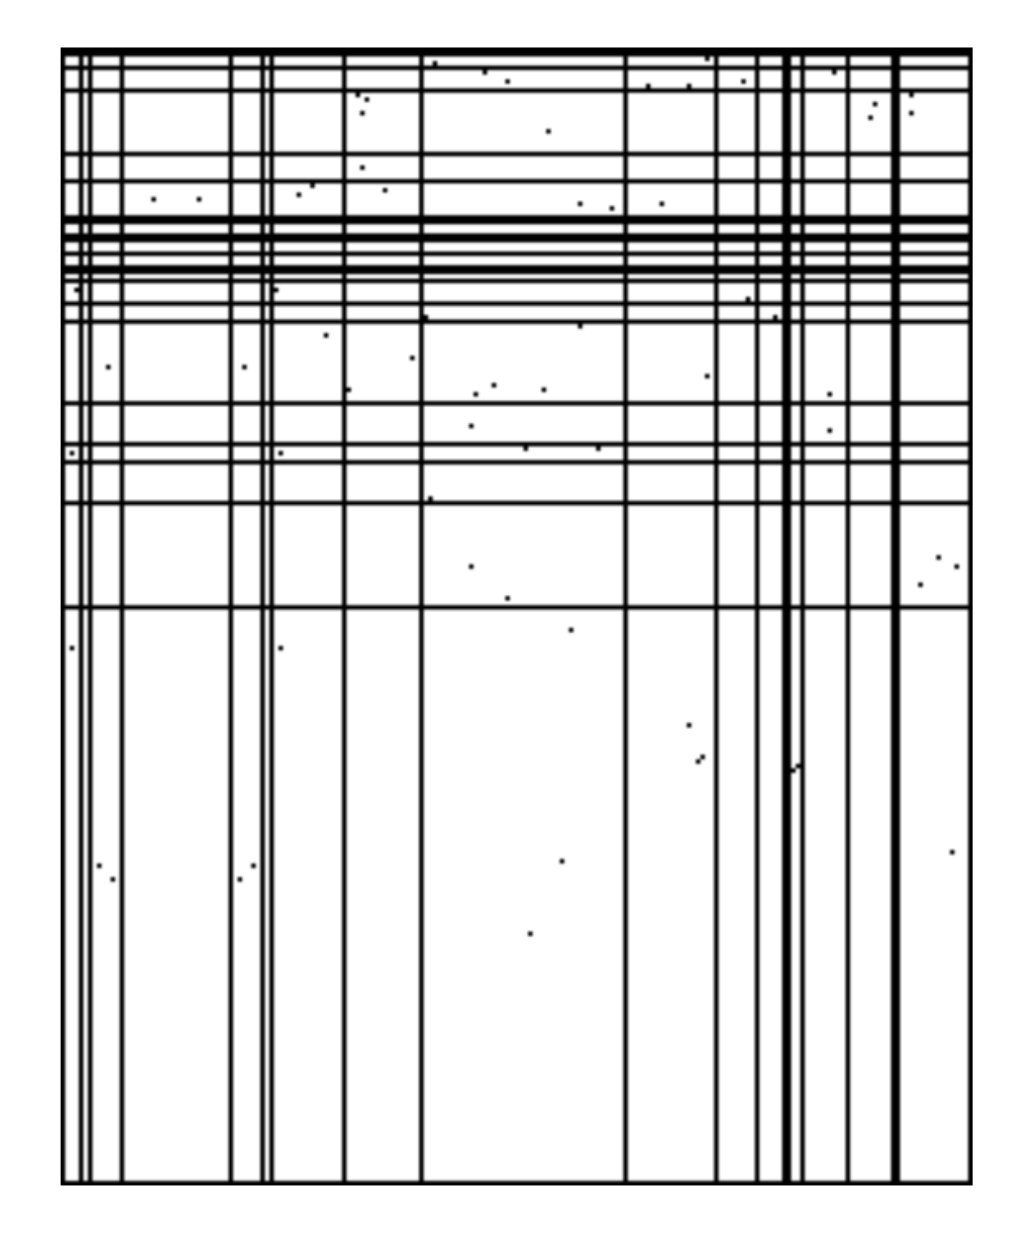
\includegraphics[width=.5\textwidth]{plot4-4}
    \caption{理想的海床分割图}
    \label{fig:plot4-4}
\end{figure}
\FloatBarrier

在划分平面之后,仍然可以利用上面的算法分别计算需要的变量,不多赘述。

\section{模型优缺点}
\subsection{模型的优点}
\textbf{优点1、多角度分析:}论文在解决问题1时采用了两种不同的解法,充分利用了三角形的几何特性(正余弦定理,相似三角形),可以帮助提供更全面的理解和解决方案;

\textbf{优点2、等效坡面角的引入:}对于问题2,引入了等效坡面角的概念,使得模型更加清晰和简洁;

\textbf{优点3、动态规划思想的应用:}在问题3中,使用了动态规划的思想来解决复杂的测线走向问题,提高了方案的可行性和高效性;

\textbf{优点4、Laplace算子:}受到该算子启发,得到上下和左右两侧深度差的差的和,同时设置一个阈值,作为划分海域范围的标准;

\textbf{优点5、问题分解和可视化:}在解决问题4时,采用微元的思想将问题分解成若干个子问题,并结合可视化技巧和数理工具,有助于处理具体而复杂的平面划分问题;

\textbf{优点6、线性回归:}线性回归模型提供了每个特征对目标变量的权重,可以快速方便的拟合平面。

\subsection{模型的缺点}
\textbf{缺点1、} 在第四个问题中,仅考虑将模型拟合为四个平面的情况,可能相对于原始海平面来说过于简化;

\textbf{缺点2、} 问题三没有充分考虑曲线航道的情况,尽管在前文的分析中排除了这种情况,但由于未进行定量计算,仍可能存在局限性,无法全面找出最优解的解决方案。

%参考文献
\begin{thebibliography}{9}%宽度9
    \bibitem[1]{ref1}
    吴自银, 阳凡林, 罗孝文, 等.
    \newblock 高分辨率海底地形地貌——探测处理理论与技术\allowbreak[M].
    \newblock 北京: 科学出版社, 2017.
    \bibitem[2]{ref2}
    王风帆,马永.
    \newblock 极地海洋多波束测量测线布设系统设计及实现\allowbreak[J].
    \newblock 海洋信息技术与应用, 2023, 38(3): 158-162.
\end{thebibliography}

\newpage
%附录
\begin{appendices}

\section{表格批量填充(Python源代码)}
\noindent 这是问题1的表格批量填充代码:
\begin{tcode}
import math
import pandas as pd

def calculate():
    # 定义参数
    D_center = 70  # 中心点的深度
    theta = math.radians(120)  # 换能器开角转换为弧度
    alpha = math.radians(1.5)  # 坡度角转换为弧度
    d = 200  # 相邻两条测线的间距
    distances_from_center = [-800, -600, -400, -200, 0, 200, 400, 600, 800]

    # 根据距中心的距离计算每个位置的深度、覆盖宽度和与前一条测线的重叠率
    depths_list = []
    coverage_widths_list = []
    overlap_percentages_list = []

    previous_width = None
    for dist in distances_from_center:
        # 修改了此行,使其与距离的正负符号相反
        D = D_center - dist * math.tan(alpha)
        depths_list.append(D)

        W_prime = D * math.sin(theta/2) / math.cos(theta/2 - alpha) \
        					+ (D - d * math.tan(alpha) * math.sin(theta/2)) / \ 
                            math.cos(theta/2 + alpha) - d / math.cos(alpha)
        coverage_widths_list.append(W_prime)

        if previous_width is not None:
            overlap = 1 - d / (2 * D) * (1 / math.tan(theta / 2) + math.tan(alpha))
            overlap_percentages_list.append(overlap * 100)
        else:
            overlap_percentages_list.append(0)  # 第一个点的重叠率为0
        previous_width = W_prime

    # 结果存储到DataFrame
    df_result10 = pd.DataFrame({
        '测线距中心点处的距离/m': distances_from_center,
        '海水深度/m': depths_list,
        '覆盖宽度/m': coverage_widths_list,
        '与前一条测线的重叠率/%':overlap_percentages_list
    })
    # 保存结果到Excel文件
    file_path = "../data/result1.xlsx"
    df_result10.to_excel(file_path, index=False)
    print(f"结果已保存到 {file_path}")

if __name__ == "__main__":
    calculate()
\end{tcode}

\noindent 这是问题2的表格批量填充代码:
\begin{tcode}
# 导入必要的库
import numpy as np
import pandas as pd
from numpy import pi as pi
from numpy import sin as sin
from numpy import cos as cos
from numpy import tan as tan
from numpy import arctan as act

# 设置pandas的显示选项,使其能够显示所有的列和行
pd.set_option('display.max_columns', None)
pd.set_option('display.max_rows', None)

# 定义常数
sp = np.deg2rad(1.5)  # 将1.5度转换为弧度

# 定义函数get_width,用于计算宽度
def get_width(beta, length):
    depth = 120 - length * sin(beta - pi/2) * tan(sp)
    alpha = act(sin(beta) * tan(sp))
    cf = depth * sin(pi / 3) / cos(pi/3 + alpha) + depth * sin(pi / 3) / cos(pi/3 - alpha)
    return cf

# 定义输入角度和长度的数组
angle = np.array([0, pi/4, pi/2, 3*pi/4, pi, 5*pi/4, 3*pi/2, 7*pi/4])
angle_string = np.array(['0', 'pi/4', 'pi/2', '3*pi/4', 'pi', '5*pi/4', '3*pi/2', '7*pi/4'])
length = np.array([0, 0.3, 0.6, 0.9, 1.2, 1.5, 1.8, 2.1]) * 1852  # 1852是海里到米的转换系数

# 初始化一个8x8的矩阵来存储结果
graph = np.zeros((8, 8))

# 用双重循环计算每个角度和长度组合的宽度
for m in range(0, 8):
    for n in range(0, 8):
        graph[m, n] = round(get_width(angle[m], length[n]))

# 将结果矩阵转换为DataFrame,以便于查看和保存
df = pd.DataFrame(graph, index=angle_string, columns=length/1852)

# 打印DataFrame
print(df)

# 将DataFrame保存为CSV文件
df.to_csv('data.csv')
\end{tcode}

\section{矩形海域侧线规划与方案可视化代码(Python源代码)}
\noindent 这是矩形海域侧线规划与方案可视化代码:
\begin{tcode}
import numpy as np
from scipy.optimize import root
from numpy import pi as pi
import matplotlib.pyplot as plt

# 初始化深度数据
center_depth = 110
west_depth = 110 + 2 * 1852 * np.tan(np.deg2rad(1.5))
east_depth = 110 - 2 * 1852 * np.tan(np.deg2rad(1.5))

def compute_distance_from_east_to_west():
    """从东向西计算船的检测线距离"""
    # 初始化船的位置
    def first_depth(x):
        return -(x * np.sin(pi/3)) / np.cos(pi/3 - np.deg2rad(1.5)) * np.sin(np.deg2rad(1.5)) + x - east_depth

    def get_d(x):
        return 1 + (x / (2 * D)) * (-1/np.tan(pi/3) + np.tan(np.deg2rad(1.5))) - 0.1

    def get_fj(x):
        return (x * np.sin(pi/3) / np.cos(pi/3 + np.deg2rad(1.5))) * np.cos(np.deg2rad(1.5))

    x0 = 110
    result = root(first_depth, x0)
    first_depth_west = result.x[0]
    first_d = first_depth_west * np.sin(pi/3) * np.cos(np.deg2rad(1.5)) / np.cos(pi/3 + np.deg2rad(1.5))
    d_sum = first_d
    D = first_depth_west
    n = 1
    distance_list = [d_sum]
    while d_sum + get_fj(D) <= 4 * 1852:
        result = root(get_d, 100)
        new_d = result.x[0]
        d_sum += new_d
        distance_list.append(d_sum)
        D = east_depth + d_sum * np.tan(np.deg2rad(1.5))
        n += 1

    print('从东向西一共有', n, '条测线,总路程为', n * 2 * 1852, '米', n * 2, '海里')
    return distance_list

def compute_distance_from_west_to_east():
    """从西向东计算船的检测线距离"""
    # 初始化船的位置
    def first_depth(x):
        return ((x*np.sin(pi/3)) / np.cos(pi/3 + np.deg2rad(1.5))) * np.sin(np.deg2rad(1.5)) + x - west_depth

    def get_d(x):
        return 1 - (x / (2 * D)) * (1/np.tan(pi/3) + np.tan(np.deg2rad(1.5))) - 0.1

    def get_fj(x):
        return (x * np.sin(pi/3) / np.cos(pi/3 - np.deg2rad(1.5))) * np.cos(np.deg2rad(1.5))

    x0 = 110
    result = root(first_depth, x0)
    first_depth_west = result.x[0]
    first_d = first_depth_west * np.sin(pi/3) * np.cos(np.deg2rad(1.5)) / np.cos(pi/3 + np.deg2rad(1.5))
    d_sum = first_d
    D = first_depth_west
    n = 1
    distance_list = [d_sum]
    while d_sum + get_fj(D) <= 4 * 1852:
        result = root(get_d, 100)
        new_d = result.x[0]
        d_sum += new_d
        distance_list.append(d_sum)
        D = west_depth - d_sum * np.tan(np.deg2rad(1.5))
        n += 1

    print('从西向东一共有', n, '条测线,总路程为', n * 2 * 1852, '米', n * 2, '海里')
    return distance_list

# 计算从东向西和从西向东的船的检测线距离
distance_list_east = compute_distance_from_east_to_west()
distance_list_west = compute_distance_from_west_to_east()

# 具体参数
print("东起", distance_list_east)
print("西起", distance_list_west)

# 创建图形显示结果
fig, ax = plt.subplots()

# 绘制从东向西的检测线
x = [0, 2]
for item in distance_list_east:
    y = [4 - item / 1852, 4 - item / 1852]
    ax.plot(x, y, color='red', linewidth=1)

# 绘制从西向东的检测线
for item in distance_list_west:
    y = [item / 1852, item / 1852]
    ax.plot(x, y, color='blue', linewidth=1)

ax.set_xlim(0, 2)
ax.set_ylim(0, 4)
ax.set_aspect(1)
plt.show()
\end{tcode}

\section{海底地形图3D图和热力图(Python源代码)}
\noindent 这是3D图的可视化代码:
\begin{tcode}
from mpl_toolkits.mplot3d import Axes3D

# Create X and Y coordinates
x = np.linspace(0, 4, depth_data.shape[1])
y = np.linspace(0, depth_data.shape[0]*0.02, depth_data.shape[0])
X, Y = np.meshgrid(x, y)

# Plot 3D sea depth distribution
fig = plt.figure(figsize=(12, 8))
ax = fig.add_subplot(111, projection='3d')
surf = ax.plot_surface(X, Y, depth_data, cmap='plasma', edgecolor='none')
ax.set_title('3D 海底深度分布')
ax.set_xlabel('横向坐标/NM(由西向东)')
ax.set_ylabel('纵向坐标/NM(由南向北)')
ax.set_zlabel('海水深度/m')
fig.colorbar(surf, ax=ax, pad=0.01, label='海水深度/m')
plt.tight_layout()
plt.show()
\end{tcode}

\noindent 这是热力图的可视化代码:
\begin{tcode}
# Create the heatmap using the 'plasma' colormap
plt.figure(figsize=(10, 8))
plt.imshow(depth_data, cmap='plasma', aspect='auto')
plt.colorbar(label='海水深度/m')
plt.title('海底深度热力图')
plt.xlabel('横向坐标/NM(由西向东)')
plt.ylabel('纵向坐标/NM(由南向北)')
plt.tight_layout()
plt.show()
\end{tcode}

\section{海底地形图划分、规划路线和指标计算代码(Python源码)}
\begin{tcode}
import numpy as np
import pandas as pd
import matplotlib.pyplot as plt
from numpy import pi as pi
from scipy.optimize import root


def plan(deep, alpha, limit, __x, __y, __z, direction):
    def first_depth(x):
        # try to initialize the starting location of the ship
        return ((x * np.sin(pi / 3)) / np.cos(pi / 3 + alpha)) * np.sin(alpha) + x - deep

    def get_d(x):
        # hold overlap rate to the least value 0.1 to get to the largest step length
        yita = 1 - (x / (2 * D)) * (1 / np.tan(pi / 3) + np.tan(alpha)) - 0.1
        return yita

    def get_fj(x):
        # get the remaining length of the detection and use it to test if mission is accomplished
        return (x * np.sin(pi / 3) / np.cos(pi / 3 - alpha)) * np.cos(alpha)

    # get the depth of the first detection
    x0 = 30
    result = root(first_depth, x0)

    # get its distance the west edge
    first_depth_west = result.x[0]
    first_d = first_depth_west * np.sin(pi / 3) * np.cos(alpha) / np.cos(pi / 3 + alpha)
    # set the initial length
    d_sum = first_d
    D = first_depth_west
    n = 1
    distance_list = [d_sum]

    # iteration, begin!
    while d_sum + get_fj(D) <= limit * 1852:  # stop if the distance is larger than 4
        # step1 get new d between detecting lines
        result = root(get_d, 30)
        new_d = result.x[0]
        # step2 calculate the distance to the west edge
        d_sum += new_d
        distance_list.append(d_sum)
        # step3 calculate the new depth
        D = deep - d_sum * np.tan(alpha)
        n += 1

    # print out the outcome
    if limit == 2:
        width = 2.5
    else:
        width = 2
    print('一共有', n, '条测线,总路程为', n * width * 1852, '米', n * width, '海里', '遗漏率为', missing(__x, __y, __z, direction, distance_list))
    # 创建一个新的图形对象
    fig, ax = plt.subplots()

    # 绘制南北向的线
    x = [0, 2.5]  # x坐标,这里假设示意图的宽度是1
    for item in distance_list:
        y = [item / 1852, item / 1852]  # y坐标,这里假设示意图的高度是1,线条位于垂直方向的中间位置
        ax.plot(x, y, color='green', linewidth=1)  # 设置线条的颜色为红色,线宽为2

    # 设置图形对象的属性
    ax.set_xlim(0, 2.5)
    ax.set_ylim(0, 2.1)
    ax.set_aspect(1)


def missing(__x, __y, __z, direction, d_list):
    d_list = np.array(d_list)
    missing_number = 0
    if direction == 'x':
        d_list += (__x[0] - 0.02) * 1852
        for i in range(len(__x)):
            xx = __x[i] * 1852
            zz = __z[i]
            for index in range(len(d_list) - 1):
                if d_list[index] < xx < d_list[index + 1]:
                    if zz / (xx - d_list[index]) < np.tan(pi/6) and zz / (d_list[index + 1] - xx) < np.tan(pi/6):
                        missing_number += 1
                    break
                else:
                    continue
    else:
        d_list += (__y[0] - 0.02) * 1852
        for i in range(len(__x)):
            yy = __y[i] * 1852
            zz = __z[i]
            for index in range(len(d_list) - 1):
                if d_list[index] < yy < d_list[index + 1]:
                    if zz / (yy - d_list[index]) < np.tan(pi / 6) and zz / (d_list[index + 1] - yy) < np.tan(pi / 6):
                        missing_number += 1
                    break
                else:
                    continue
    return missing_number / len(__x)


def get_angle(pa, pb):
    # 计算拟合面的法向量
    normal_vector = np.array([pa, pb, -1])  # 拟合面的法向量为(a, b, -1)

    # 水平面法向量(假设为竖直向上的)
    horizontal_vector = np.array([0, 0, 1])

    # 计算法向量之间的夹角
    cosine_angle = np.dot(normal_vector, horizontal_vector) / (
        np.linalg.norm(normal_vector) * np.linalg.norm(horizontal_vector)
    )
    angle_in_radians = np.arccos(cosine_angle)
    if angle_in_radians >= 3:
        return pi - angle_in_radians
    else:
        return angle_in_radians


df = pd.read_excel('/Users/zhangshuhan/Desktop/副本附件(1).xls', engine='xlrd')
matrix = np.array(df.values[0:, 1:])
x = matrix[0, 1:]
y = matrix[1:, 0]
z = matrix[1:, 1:]
X = []
Y = []
Z = []
for m, _x in enumerate(x):
    if m == 100:
        break
    for n, _y in enumerate(y):
        if n == 125:
            break
        X.append(_x)
        Y.append(_y)
        Z.append(z[n, m])
# 进行线性回归拟合
A = np.column_stack([X, Y, np.ones_like(X)])
coefficients, residuals, _, _ = np.linalg.lstsq(A, Z, rcond=-1)
# 提取回归系数
a, b, c = coefficients
# 生成拟合的平面面点坐标
x_fit = np.linspace(min(X), max(X), 10)
y_fit = np.linspace(min(Y), max(Y), 10)
x_fit, y_fit = np.meshgrid(x_fit, y_fit)
z_fit = a * x_fit + b * y_fit + c

# 绘制原始数据的散点图
fig = plt.figure()
ax = fig.add_subplot(111, projection='3d')

angle = get_angle(a / 1852, b / 1852)
depth = a * 2 + b * 1.25 + c
print('blue')
plan(depth, angle, limit=2, __x=X, __y=Y, __z=Z, direction='x')
# 绘制拟合的平面
ax.plot_surface(x_fit, y_fit, z_fit, color='blue', alpha=0.5, label='Fitted Plane')


X = []
Y = []
Z = []
for m, _x in enumerate(x[100:]):
    for n, _y in enumerate(y[:125]):
        X.append(_x)
        Y.append(_y)
        Z.append(z[n, m + 100])
# 进行线性回归拟合
A = np.column_stack([X, Y, np.ones_like(X)])
coefficients, residuals, _, _ = np.linalg.lstsq(A, Z, rcond=-1)

# 提取回归系数
a, b, c = coefficients

# 生成拟合的平面面点坐标
x_fit = np.linspace(min(X), max(X), 10)
y_fit = np.linspace(min(Y), max(Y), 10)
x_fit, y_fit = np.meshgrid(x_fit, y_fit)
z_fit = a * x_fit + b * y_fit + c

angle = get_angle(a / 1852, b / 1852)
depth = a * 4 + b * 1.25 + c
print('green')
plan(depth, angle, limit=2, __x=X, __y=Y, __z=Z, direction='x')


# 绘制拟合的平面
ax.plot_surface(x_fit, y_fit, z_fit, color='green', alpha=0.5, label='Fitted Plane')


X = []
Y = []
Z = []
for m, _x in enumerate(x[:100]):
    for n, _y in enumerate(y[125:]):
        X.append(_x)
        Y.append(_y)
        Z.append(z[n + 125, m])
# 进行线性回归拟合
A = np.column_stack([X, Y, np.ones_like(X)])
coefficients, residuals, _, _ = np.linalg.lstsq(A, Z, rcond=-1)

# 提取回归系数
a, b, c = coefficients

# 生成拟合的平面面点坐标
x_fit = np.linspace(min(X), max(X), 10)
y_fit = np.linspace(min(Y), max(Y), 10)
x_fit, y_fit = np.meshgrid(x_fit, y_fit)
z_fit = a * x_fit + b * y_fit + c

angle = get_angle(a / 1852, b / 1852)
depth = a * 1 + b * 5 + c
print('red')
plan(depth, angle, limit=2.5, __x=X, __y=Y, __z=Z, direction='y')


# 绘制拟合的平面
ax.plot_surface(x_fit, y_fit, z_fit, color='red', alpha=0.5, label='Fitted Plane')


X = []
Y = []
Z = []
for m, _x in enumerate(x[100:]):
    for n, _y in enumerate(y[125:]):
        X.append(_x)
        Y.append(_y)
        Z.append(z[n + 125, m + 100])
# 进行线性回归拟合
A = np.column_stack([X, Y, np.ones_like(X)])
coefficients, residuals, _, _ = np.linalg.lstsq(A, Z, rcond=-1)

# 提取回归系数
a, b, c = coefficients

# 生成拟合的平面面点坐标
x_fit = np.linspace(min(X), max(X), 10)
y_fit = np.linspace(min(Y), max(Y), 10)
x_fit, y_fit = np.meshgrid(x_fit, y_fit)
z_fit = a * x_fit + b * y_fit + c

angle = get_angle(a / 1852, b / 1852)
depth = a * 4 + b * 3.75 + c
print('yellow')
plan(depth, angle, limit=2, __x=X, __y=Y, __z=Z, direction='x')


# 绘制拟合的平面
ax.plot_surface(x_fit, y_fit, z_fit, color='yellow', alpha=0.5, label='Fitted Plane')


# 设置坐标轴标签
ax.set_xlabel('X')
ax.set_ylabel('Y')
ax.set_zlabel('Z')
# 显示图像
# plt.show()
\end{tcode}

\end{appendices}
\end{document} 